\documentclass[12pt]{article}

\usepackage{graphicx}
\usepackage{fullpage}
\usepackage{relsize}
\usepackage{amssymb}
\usepackage{dirtytalk}
\usepackage{amsmath, mathtools}
\usepackage{braket}
\usepackage[x11names]{xcolor}
\usepackage{hyperref}
\usepackage{tcolorbox}
\usepackage{ dsfont }
\usepackage{enumitem}
\usepackage{natbib}
\usepackage{ wasysym }
\usepackage{amsthm}
\usepackage{ gensymb }
\newtheorem{theorem}{Theorem}[section]
\newtheorem{lemma}[theorem]{Lemma}
\definecolor{mytheorembg}{HTML}{F2F2F9}
\definecolor{mytheoremfr}{HTML}{00007B}
\definecolor{myexamplebg}{HTML}{F2FBF8}
\definecolor{myexamplefr}{HTML}{88D6D1}
\definecolor{myexampleti}{HTML}{2A7F7F}
\definecolor{mydefinitbg}{HTML}{E5E5FF}
\definecolor{mydefinitfr}{HTML}{3F3FA3}
\newtcbox{\mybox}{on line,
  colframe=black,colback=Chartreuse1,
  boxrule=0.5pt,arc=4pt,boxsep=0pt,left=6pt,right=6pt,top=6pt,bottom=6pt}
  \newtcbox{\myboxs}{on line,
  colframe=black,colback=Red1!40!white,
  boxrule=0.5pt,arc=4pt,boxsep=0pt,left=6pt,right=6pt,top=6pt,bottom=6pt}
\tcbuselibrary{theorems,skins,hooks}
\newtcbtheorem[number within=section]{Theorem}{Theorem}
  {%
     enhanced
    ,colback = mytheorembg
    ,frame hidden
    ,boxrule = 0sp
    ,borderline west = {2pt}{0pt}{mytheoremfr}
    ,sharp corners
    ,detach title
    ,before upper = \tcbtitle\par\smallskip
    ,coltitle = mytheoremfr
    ,fonttitle = \bfseries\sffamily
    ,description font = \mdseries
    ,terminator sign dash
    ,separator sign none
  }
  {th}
\newtcbtheorem[number within=section]{Example}{Example}
  {%
     colback = myexamplebg
    ,colframe = myexamplefr
    ,coltitle = myexampleti
    ,boxrule = 1pt
    ,sharp corners
    ,detach title
    ,before upper=\tcbtitle\par\smallskip
    ,fonttitle = \bfseries
    ,description font = \mdseries
    ,separator sign none
    ,description delimiters parenthesis
  }
  {ex}
\newtcolorbox{Definition}[1]
  {
     enhanced
    ,colback = mydefinitbg
    ,colframe = mydefinitfr
    ,coltitle = mydefinitfr
    ,colbacktitle = mydefinitbg
    ,fonttitle = \bfseries
    ,title = {#1}
    ,attach boxed title to top right = {yshift = -5pt, xshift = -7mm}
    ,boxed title style = { boxrule = .25mm }
    ,arc = 5mm
    ,interior code app =
      {
        \node
          [
             anchor=south west
            ,line width = 0.5mm
            ,rounded corners
            ,inner sep = 5pt
            ,draw = mydefinitfr
            ,fill = mydefinitbg
            ,yshift = -5pt%3.5pt
            ,xshift = 7mm
            ,text = mydefinitfr
            ,font = \bfseries
          ] at (frame.north west)
          {\ Definition\ \null};
      }
  }
\setlength{\parindent}{0cm}

\title{IGMO 2020 Shortlist}
\author{IGMO 2020 Team }
\date{December}

\begin{document}

\maketitle

\begin{center}
    \quad \quad 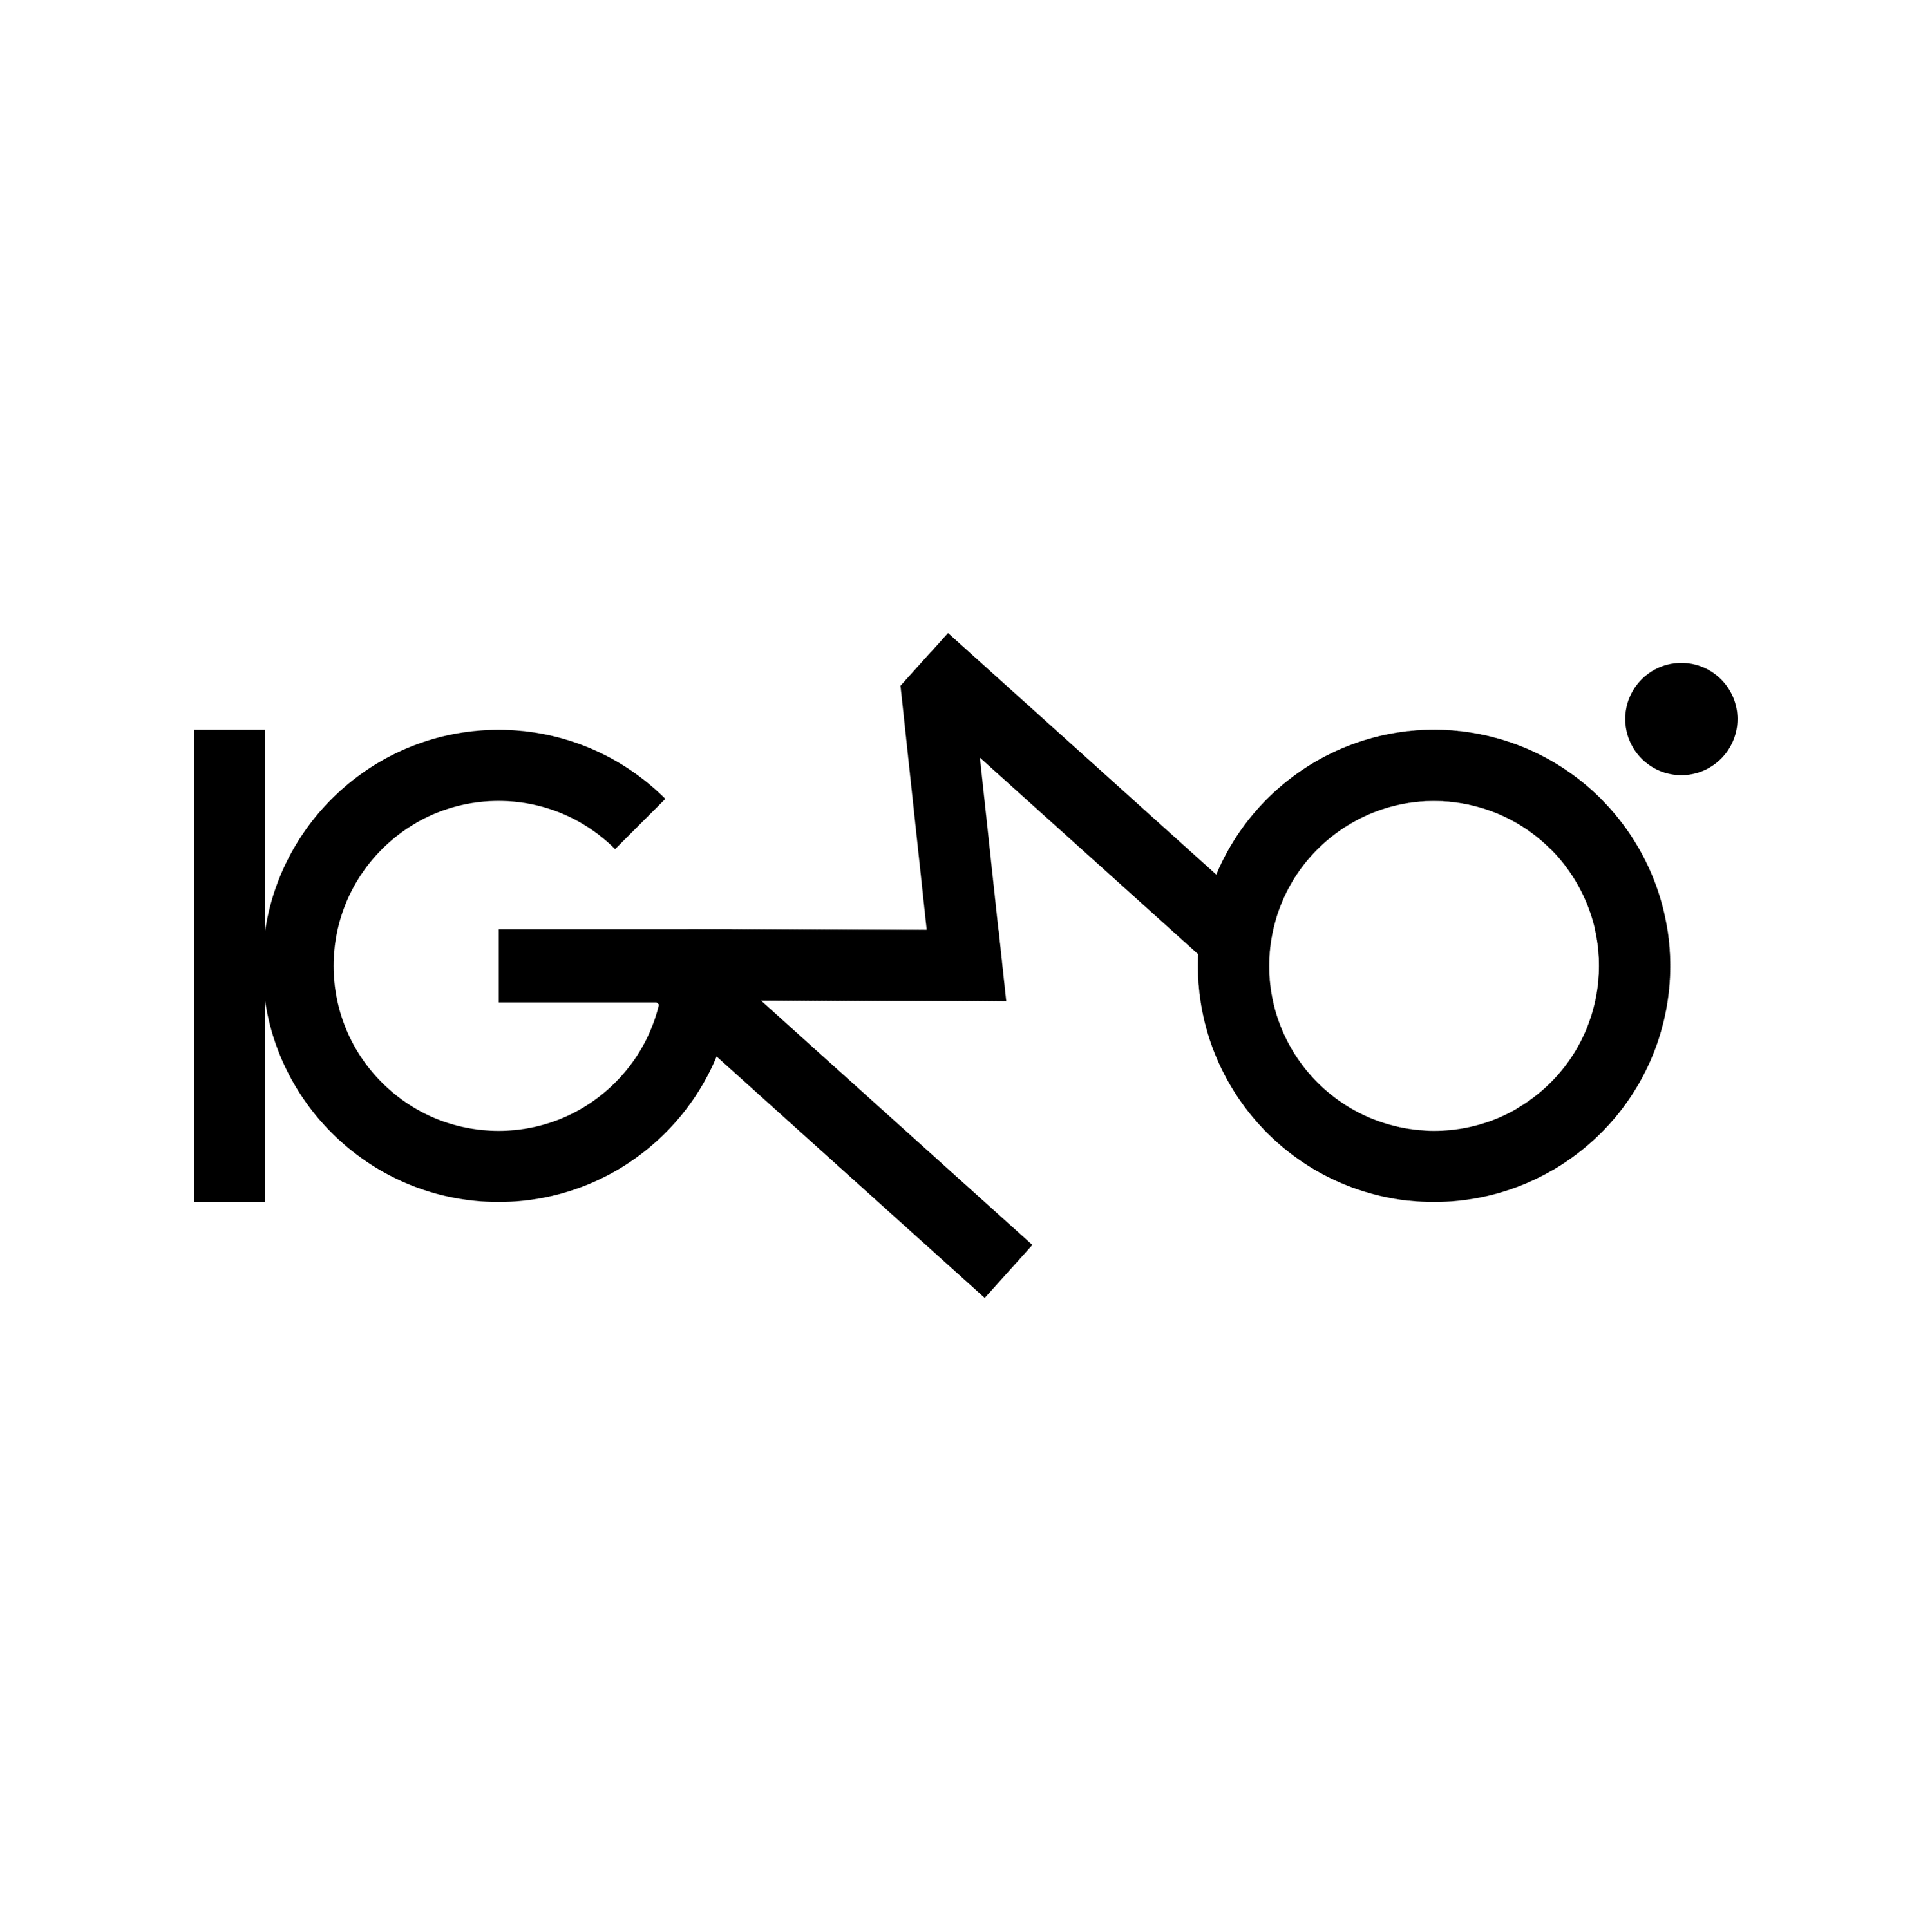
\includegraphics[width = 8cm]{IGMO_SIGMA png (2).png}
\end{center}
\newpage







\newpage

%This is the 2nd page, try to mkae this like IMO SL%

\begin{center}
    \section*{2nd Page}
\end{center}

\newpage



%This is the 3rd page(after this problems will come%

{\LARGE
\begin{center}
\section*{\huge{\underline{Round 1 Problems}}}
    \mybox{\hyperlink{R1P1}{Round 1 P1}} \\ \vspace{4mm}
    \mybox{Round 1 P2} \\ \vspace{4mm}
    \mybox{Round 1 P3} \\ \vspace{4mm}
    \mybox{Round 1 P4} \\ \vspace{4mm}
    \mybox{Round 1 P5} \\ \vspace{4mm}
    \mybox{Round 1 P6} \\  \vspace{4mm}
\section*{\huge{\underline{Round 2 Problems}}}
    \mybox{Round 2 P1} \\ \vspace{4mm}
    \mybox{Round 2 P2} \\ \vspace{4mm}
    \mybox{Round 2 P3} \\ \vspace{4mm}
    \mybox{Round 2 P4} \\ \vspace{4mm}
    \mybox{Round 2 P5} \\ \vspace{4mm}
    \mybox{Round 2 P6} \\ \vspace{4mm}
\end{center}
}







\newpage

\section*{Algebra}
\mybox{\hypertarget{R1P1}{Problem 1 : }} Prove the inequality which states that if you let $x_{1}, x_{2}, \ldots, x_{n}$ be positive real numbers, with $n \geq 2,$ then you have the inequality
$$
\frac{x_{1}}{x_{2}+x_{3}+\cdots+x_{n}}+\frac{x_{2}}{x_{1}+x_{3}+x_{4}+\cdots+x_{n}}+\cdots+\frac{x_{n}}{x_{1}+x_{2}+\cdots+x_{n-1}} \geq \frac{n}{n-1}
$$
\begin{flushright}
\textbf{Problem posed by}
\textcolor{RoyalBlue2}{\href{https://www.instagram.com/creative_math_/}{@creative\_math\_}}
\end{flushright}





\subsection*{\myboxs{Solution : }}
We'll use Chebyshev's inequality here. WLOG we can assume that $x_1\leq x_2\leq \cdots x_{n-1} \leq x_n$ and then set $a_k = x_k$. From this we also know that 
$$ \frac{1}{x_2+x_3+\cdots+x_{n-1}+x_n} \leq \frac{1}{x_1+x_3+\cdots+x_{n-1}+x_n} \leq \cdots \leq \frac{1}{x_1+x_2+\cdots+x_{n-1}}   $$
and we can set our $b_k$ to be these expressions as so $$b_k  \times \sum_{i \in \mathbb{N} / \{k\} } x_i = 1$$
Both $a_k$ and $b_k$ are increasing sequences so we can apply Chebyshev's inequality to give
$$ n\sum a_kb_k \geq \left( \sum a_k \right) \left(\sum b_k  \right) \Rightarrow n I \geq n + I $$
Where $I$ is the inequality expression (you can obtain $n+I$ after expanding the product)
$$ \therefore I \geq \frac{n}{n-1}$$
\begin{flushright}
\textbf{7 marks}
\end{flushright}

Of course, any other valid method can be used and that secures marks too.  
 \subsection*{\mybox{Problem 2 :}}
 Let $a_1$, $a_2$, $b_2$, $b_3$, $c_1$, $c_2$ be positive numbers such that $a_1 b_1 - c_1 ^2 >0$ and  $a_2 b_2 - c_2 ^2 >0$. Prove that $$\frac{8}{(a_1+a_2)(b_1+b_2)-{(c_1+c_2)}^2}\le\frac{1}{a_1b_1-{c_1}^2}+\frac{1}{a_2b_2-{c_2}^2}$$
 
 \begin{flushright}
\textbf{Problem posed by}
\textcolor{RoyalBlue2}{\href{https://www.instagram.com/pepemaths/}{@pepemaths}}
\end{flushright}

 
 
 
 
 
 \subsection*{\myboxs{Solution : }}

Let $D_1=a_1b_1-{c_1}^2$ and $D_2=a_2b_2-{c_2}^2$.
$$\frac{8}{(a_1+a_2)(b_1+b_2)-{(c_1+c_2)}^2}-\frac{1}{a_1b_1-{c_1}^2}-\frac{1}{a_2b_2-{c_2}^2}$$
$$=\frac{8}{a_1b_1-{c_1}^2+a_2b_2-{c_2}^2+a_1b_2+a_2b_1-2c_1c_2}-\frac{1}{a_1b_1-{c_1}^2}-\frac{1}{a_2b_2-{c_2}^2}$$
$$=\frac{8}{D_1+D_2+a_1b_2+a_2b_1-2c_1c_2}-\frac{1}{D_1}-\frac{1}{D_2}$$
$$\le\frac{8}{D_1+D_2+a_1b_2+a_2b_1-(\frac{b_2{c_1}^2}{b_1}+\frac{b_1{c_2}^2}{b_2})}-\frac{1}{D_1}-\frac{1}{D_2}$$
$$=\frac{8}{(D_1+D_2)+(\frac{b_2}{b_1}D_1+\frac{b_1}{b_2}D_2)}-\frac{1}{D_1}-\frac{1}{D_2}$$
$$\le\frac{8}{2\sqrt{D_1D_2}+2\sqrt{D_1D_2}}-\frac{1}{D_1}-\frac{1}{D_2}$$
$$=\frac{2}{\sqrt{D_1D_2}}-\frac{1}{D_1}-\frac{1}{D_2}=-{(\frac{1}{\sqrt{D_1}}-\frac{1}{\sqrt{D_2}})}^2\le0$$

So $$\frac{8}{(a_1+a_2)(b_1+b_2)-{(c_1+c_2)}^2}\le\frac{1}{a_1b_1-{c_1}^2}+\frac{1}{a_2b_2-{c_2}^2}$$
\begin{flushright}
\textbf{7 marks}
\end{flushright}

\subsection*{\mybox{Problem 3 :}}
Find all $f: \mathbb{Q}^{+} \rightarrow \mathbb{Q}^{+}$ satisfying:
 $$ \textmd{(a) } f(x)+f\left(\frac{1}{x}\right)=1, \textmd{ for all x} \in \mathbb{Q}^{+}$$ 
  $$ \textmd{(b) }f(1+2 x)=\frac{1}{2} f(x), \textmd{ for all x} \in \mathbb{Q}^{+}$$ \\
\textbf{proving} that you have found all such $f : \mathbb{Q}^{+} \rightarrow \mathbb{Q}^{+}$





\begin{flushright}
\textbf{Problem posed by} 
\textcolor{RoyalBlue2}{\href{https://www.instagram.com/creative.math_solving/}{@creative.math\_solving}}
\end{flushright}








\subsection*{\myboxs{Solution :}}
Taking $x=1$ in $(\mathrm{a}),$ we get $f(1)=1 / 2$. If we set $x=1 / 2$ in $(\mathrm{a})$ and $(\mathrm{b}),$ we see that
$$
f\left(\frac{1}{2}\right)+f(2)=1 ;\quad f(2)=\frac{1}{2} f\left(\frac{1}{2}\right)
$$
Solving for $f(2)$ and $f\left(\frac{1}{2}\right),$ we obtain
$$
f(2)=\frac{1}{3},\quad f\left(\frac{1}{2}\right)=\frac{2}{3}
$$
Taking $x=1$ in $($b$),$ we see that
$$
f(3)=\frac{1}{2} f(1)=\frac{1}{4}
$$
Now if we use (a), we compute
$$
f\left(\frac{1}{3}\right)=1-f(3)=\frac{3}{4}
$$
Similarly substituting $x=1 / 4$ in $(b)$ we see that
$$
f\left(\frac{3}{2}\right)=\frac{1}{2} f\left(\frac{1}{4}\right)
$$and taking $x=3 / 2$ in (a) we obtain
$$
f(4)=\frac{1}{2} f\left(\frac{3}{2}\right)
$$
If we eliminate $f\left(\frac{3}{2}\right)$ from these two relations, we get
$$
f(4)=\frac{1}{4} f\left(\frac{1}{4}\right)
$$
But we know from (a) that
$$
f(4)+f\left(\frac{1}{4}\right)=1
$$
It follows that
$$
f(4)=\frac{1}{5}, \quad \text { and } \quad f\left(\frac{1}{4}\right)=\frac{4}{5}
$$
These in turn leads to
$$
f\left(\frac{3}{2}\right)=\frac{2}{5}, \text { and } f\left(\frac{2}{3}\right)=\frac{3}{5}
$$

An inspection of the values so far obtained reveals that $f(x)=\dfrac{1}{1+x}$ is possibly the required function. We show that this indeed is the solution of our functional equation. We adopt the following procedure to prove our claim by induction. For each rational $r=p / q \in \mathbb{Q}^{+}$ with $gcd(p, q)= 1$, we define $d(r)=p+q$ which is a natural number. We show that $f(r)=\frac{1}{1+r}$ by using induction on $d(r)$. We have so far verified this claim for all $r \in \mathbb{Q}^{+}$ for which $d(r) \leq 5$ holds.

Suppose this result is true for all $r \in \mathbb{Q}^{+}$ such that $d(r) \leq$
$N .$ Take any $r=p / q \in \mathbb{Q}^{+}$ such that $gcd(p, q)=1$ and $d(r)=p+q=N+1 .$ We have
$$
f\left(\frac{q}{p}\right)=f\left(1+2\left(\frac{q-p}{2 p}\right)\right)=\frac{1}{2} f\left(\frac{q-p}{2 p}\right)
$$If $q$ and $p$ are both odd, then 2 divides $q-p .$ Thus
$$
d\left(\frac{q-p}{2 p}\right) \leq \frac{q-p}{2}+p=\frac{q+p}{2} \leq N
$$
By induction hypothesis, we obtain
$$
f\left(\frac{q-p}{2 p}\right)=\frac{1}{1+\frac{q-p}{2 p}}=\frac{2 p}{q+p}
$$
Thus we get
$$
f\left(\frac{q}{p}\right)=\frac{p}{p+q}
$$
and
$$
f\left(\frac{p}{q}\right)=1-f\left(\frac{q}{p}\right)=\frac{q}{p+q}=\frac{1}{1+\frac{p}{q}}
$$
Suppose $p$ and $q$ have different parity. If $q-p>2 p,$ then
$$
f\left(\frac{q-p}{2 p}\right)=f\left(1+2\left(\frac{q-3 p}{4 p}\right)\right)=\frac{1}{2} f\left(\frac{q-3 p}{4 p}\right)
$$
and hence
$$
f\left(\frac{q}{p}\right)=\frac{1}{2} f\left(\frac{q-p}{2 p}\right)=\frac{1}{2^{2}} f\left(\frac{q-\left(2^{2}-1\right) p}{2^{2} p}\right)
$$
Let $s_{1}$ be the least positive integer such that $2^{s_{1}} p>q-\left(2^{s_{1}}-1\right) p .$ Using the above procedure we arrive at
$$
f\left(\frac{q}{p}\right)=\frac{1}{2^{s_{1}}} f\left(\frac{q-\left(2^{s_{1}}-1\right) p}{2^{s_{1} p}}\right)
$$
Put $q_{1}=2^{s_{1}} p$ and $p_{1}=q-\left(2^{s_{1}}-1\right) p .$ Then we can express $f\left(q_{1} / p_{1}\right)$ by
$$
f\left(\frac{q_{1}}{p_{1}}\right)=1-f\left(\frac{p_{1}}{q_{1}}\right)=1-2^{s_{1}} f\left(\frac{q}{p}\right)
$$We observe that
$$
d\left(\frac{q_{1}}{p_{1}}\right)=q_{1}+p_{1}=q+p=N+1
$$
and $gcd\left(p_{1}, q_{1}\right)=gcd(p, q)=1 .$ Let $s_{2}$ be the least positive integer such that
$$
2^{s_{2}} p_{1}>q_{1}-\left(2^{s_{2}}-1\right) p_{1}
$$
Then we obtain
$$
f\left(\frac{q_{1}}{p_{1}}\right)=\frac{1}{2^{s_{2}}} f\left(\frac{p_{2}}{q_{2}}\right)
$$
where $q_{2}=2^{s_{2}} p_{1}$ and $p_{2}=q_{1}-\left(2^{s_{2}}-1\right) p_{1} .$ Thus we obtain
$$
\begin{aligned}
f\left(\frac{q_{2}}{p_{2}}\right) &=1-f\left(\frac{p_{2}}{q_{2}}\right) \\
&=1-2^{s_{2}} f\left(\frac{q_{1}}{p_{1}}\right) \\
&=1-2^{s_{2}}\left(1-f\left(\frac{p_{1}}{q_{1}}\right)\right) \\
&=1-2^{s_{2}}+2^{s_{2}+s_{1}} f\left(\frac{q}{p}\right)
\end{aligned}
$$
Continuing this process, we get a sequence $\langle\left(p_{k}, q_{k}\right)\rangle$ such that
\begin{enumerate}
\item $gcd\left(p_{k}, q_{k}\right)=1$ for all $k$
\item $p_{k}+q_{k}=p+q=N+1,$ for all $k$
\item $p_{k}=q_{k-1}-\left(2^{s_{k}}-1\right) p_{k-1}$ and $q_{k}=2^{s_{k}} p_{k-1}$ ( here
$p_{0}=p$ and $q_{0}=q$ ) where $s_{k}$ is the least positive integer such that $2^{s_{k}} p_{k-1}>q_{k-1}-\left(2^{s_{k}}-1\right) p_{k-1}$
\item $2^{5_{k}} f\left(\dfrac{q_{k-1}}{p_{k-1}}\right)=f\left(\dfrac{p_{k}}{q_{k}}\right)$
\end{enumerate}

Now there are only finitely many solutions to the equation $a+b=N+1$ with $gcd(a, b)=1$. Hence there must be repetitions in the in the sequence $\left\langle\left(p_{k}, q_{k}\right)\right\rangle$. Let us suppose
$$
\left(p_{m}, q_{m}\right)=\left(p_{m+t}, q_{m+t}\right)
$$
For convenience, let us also introduce
$$
2^{s_{m+t}+s_{m+t-1}+\cdots+s_{m+t-r}}=u_{r}
$$
We then obtain
$$
\begin{aligned}
f\left(\frac{p_{m+t}}{q_{m+t}}\right) &=2^{s_{m+t}} f\left(\frac{q_{m+t-1}}{p_{m+t-1}}\right) \\
&=2^{s_{m+t}}-2^{s_{m+t}} f\left(\frac{p_{m+t-1}}{q_{m+t-1}}\right) \\
&=u_{0}-u_{1}+u_{1} f\left(\frac{p_{m+t-2}}{q_{m+t-2}}\right) \\
 & \qquad\vdots\qquad \qquad\vdots \qquad\qquad\vdots\\
&=u_{0}-u_{1}+\cdots+(-1)^{t-1} u_{t-1} +(-1)^tu_{t-1}f\left(\dfrac{p_m}{q_m}\right)
\end{aligned}
$$
Now using $p_{m+t}=p_{m}$ and $q_{m+t}=q_{m}$ we solve for $f\left(\frac{p_{m}}{q_{m}}\right):$
$$
f\left(\frac{p_{m}}{q_{m}}\right)=\frac{u_{0}-u_{1}+\cdots+(-1)^{t-1} u_{t-1}}{1-(-1)^{t} u_{t}}
$$
However, we also have
\begin{align*}
p_{m+t} &=q_{m+t-1}-\left(2^{s_{m}+t}-1\right) p_{m+t-1} \\
&=q_{m+t-1}+p_{m+t-1}-2^{s_{m+t}} p_{m+t-1} \\
&=\left(p_{m}+q_{m}\right)-2^{s_{m+t}} p_{m+t-1}
\end{align*}

An easy induction gives

\[
p_{m+t}=\left(p_{m}+q_{m}\right)\left\{1-u_{0}+u_{1}-u_{2}+\cdots+(-1)^{t-1} u_{t-2}\right\}+(-1)^{t} u_{t-1} p_{m}
\]
Using $p_{m+t}=p_{m},$ we obtain
$$
\frac{p_{m}}{p_{m}+q_{m}}=\frac{1-u_{0}+u_{1}-u_{2}+\cdots+(-1)^{t-1} u_{t-2}}{1-(-1)^{t} u_{t-1}}
$$
But we also note that
\begin{align*}
f\left(\frac{q_{m}}{p_{m}}\right) &=1-f\left(\frac{p_{m}}{q_{m}}\right) \\
&=1-\left\{\frac{u_{0}-u_{1}+u_{2}-\cdots+(-1)^{t-1} u_{t-1}}{1-(-1)^{t} u_{t-1}}\right\} \\
&=\frac{1-u_{0}+u_{1}-u_{2}+\cdots+(-1)^{t-1} u_{t-2}}{1-(-1)^{t} u_{t-1}} \\
&=\frac{p_{m}}{p_{m}+q_{m}}
\end{align*}
Thus it follows that
$$
f\left(\frac{p_{m}}{q_{m}}\right)=1-f\left(\frac{q_{m}}{p_{m}}\right)=\frac{q_{m}}{p_{m}+q_{m}}
$$
On the other hand we also observe that
$$
f\left(\frac{p_{m}}{q_{m}}\right)=2^{s_{m}} f\left(\frac{q_{m-1}}{p_{m-1}}\right)
$$
so that
\begin{align*}
f\left(\frac{q_{m-1}}{p_{m-1}}\right) &=\frac{1}{2^{s_{m}}} f\left(\frac{p_{m}}{q_{m}}\right) \\
&=\left(\frac{1}{2^{s_{m}}}\right)\left(\frac{q_{m}}{p_{m}+q_{m}}\right) \\
&=\frac{p_{m-1}}{p_{m}+q_{m}} \\
&=\frac{p_{m-1}}{p_{m-1}+q_{m-1}}
\end{align*}
This gives
$$
f\left(\frac{p_{m-1}}{q_{m-1}}\right)=1-f\left(\frac{q_{m-1}}{p_{m-1}}\right)=\frac{q_{m-1}}{p_{m-1}+q_{m-1}}
$$Continuing this process by induction, we arrive at
$$
f\left(\frac{p}{q}\right)=f\left(\frac{p_{0}}{q_{0}}\right)=\frac{q_{0}}{p_{0}+q_{0}}=\frac{q}{p+q}
$$
Thus we finally obtain
$$
f\left(\frac{p}{q}\right)=\frac{q}{p+q}=\frac{1}{1+\frac{p}{q}}
$$
showing that $f(r)=\frac{1}{1+r}$ for all positive rationals $r$









\subsection*{\mybox{Problem 4 :}}
Given that $x_1,x_2\cdots, x_k$ are positive reals such that $\displaystyle \sum_{i=1}^{k} x_i^{n-1} = k -1$, prove that 
$$ \frac{x_1^n}{x_2+x_3+\cdots + x_k} + \frac{x_2^n}{x_1+x_3+\cdots + x_k} + \cdots + \frac{x_k^n}{x_1+x_2+\cdots + x_{k-1}} \geq 1  $$


\begin{flushright}
\textbf{Problem posed by}
\textcolor{RoyalBlue2}{\href{https://www.instagram.com/creative_math_/}{@creative\_math\_}}
\end{flushright}




\subsection*{\myboxs{Solution : }}
Firstly, notice that the inequality is cyclic. This means that we can, WLOG, assume that we have a decreasing sequence of $x_i$, or in other words $x_1 \geq x_2 \geq x_3 \geq \cdots \geq x_k$. This implies 
$$ x_1^n \quad \quad   \geq \quad \quad x_2^n \quad \quad \quad \quad    \geq  \cdots \geq \quad \quad x_k^n \quad \quad   $$
$$ \frac{1}{x_2 + x_3 + \cdots + x_k} \geq \frac{1}{x_1 + x_3 + \cdots + x_k} \geq \cdots \geq \frac{1}{x_1 + x_2+  \cdots + x_{k-1}}   $$
Applying Chebyshev's Inequality gives us 
$$ kI \geq (x_1^n+x_2^n + \cdots + x_k^n) \left( \frac{1}{x_2+x_3 + \cdots+x_k} + \frac{1}{x_1+x_3 + \cdots+x_k}  + \frac{1}{x_1+x_2+\cdots+x_{k-1}}  \right)$$
Where $I$ is the expression in the original inequality. Multiplying it out, we get one $I$ and the expression on the R.H.S
$$ (k-1)S \geq \frac{x_1^n+x_2^n+\cdots+x_{k-1}^n}{x_1+x_2+\cdots+x_{k-1}} + \frac{x_2^n+x_3^n+\cdots+x_k^n}{x_2+x_3+\cdots+x_k} + \cdots   $$
We see there's $k$ terms in the R.H.S, and we can obtain an inequality for each using Chebyshev's inequality yet again if we consider 2 sequences 
$$ x_1^{n-1} \geq x_2^{n-1} \geq \cdots \geq x_k^{n-1}  $$
$$ x_1 \geq x_2 \geq \cdots \geq x_k $$
One thing to be cautious about is that each of the terms in the R.H.S contains only $(k-1)$ number of $x_i$'s, so when we set up a chebyshev inequality for one of them(let's say the first term on the L.H.S), we get 
$$ (k-1)(x_1^n+x_2^n+\cdots + x_{k-1}^n) \geq (x_1 + x_2 + \cdots +x_{k-1})(x_1^{n-1}+x_2^{n-1}+\cdots + x_{k-1}^{n-1}) $$
Rearranging, we obtain 
$$ \frac{x_1^n+x_2^n+\cdots+x_{k-1}^n}{x_1+x_2+\cdots+x_{k-1}} \geq \frac{x_1^{n-1}+x_2^{n-1}+\cdots + x_{k-1}^{n-1}}{k-1} $$
Note that we get $k$ such inequalities, and in all the inequalities except 1, an $x_i$ will be present. So if we're adding them up, we'll $(k-1)$ number of $x_i$'s and this will cancel with the $(k-1)$ in the denominator and we obtain 
$$ (k-1)S \geq x_1^{n-1}+x_2^{n-1}+ \cdots + x_k^{n-1} $$
But, as we know that $\displaystyle \sum_{i=1}^{k} x_i^{n-1} = k-1 $, we have 
$$ S \geq 1 $$



\newpage




\section*{Discrete Mathematics}






\subsection*{\mybox{Problem 1 :}}
A computer calculates the $n$th Fibonacci Number ($F_n$, where $F_n = F_{n-1}+F_{n-2}$ and $F_0 = 0$, $F_1 =1$) using \say{steps}. A step is defined to be a single calculation (this means carrying out $a + b$ when we already know $a$ and $b$ counts as one step, though if we don't know what $a$ or $b$ are, carrying out $a+b$ takes \textit{the number of steps to find $a$} + \textit{the number of steps to find $b$} + 1, with the 1 coming from calculating $a+b$). The computer can only have $F_0$ and $F_1$ permanently stored, and it has to calculate everything else all over again when a request to calculate a new Fibonacci number is made. The advantage of this process is that the \textbf{final addition step}(to add one due to calculating $a+b$) gets omitted(by some algorithmic magic). In this algorithm, the steps needed to \say{call} $F_0$ and $F_1$ (these are the only values for which a call counts as a step) are both 1. Given that the computer can only carry out simple addition of 2 numbers at most : 
\begin{itemize}
    \item Find an expression for $S(F_n)$, the number of steps taken to find $F_n$ using this approach if we can only have $F_0$ and $F_1$ stored for all $n \geq 2$ where $S(F_0) = 1$ and $S(F_1) = 1$ due to the \say{calling} feature
    \item Find an expression for $\gcd(S(F_n),S(F_m)))$ involving only $n,m$ and the $\gcd$ function for $n,m \geq 2$
\end{itemize}
Now, the computer has the ability to \say{cache} (store) all previously calculated Fibonacci Numbers, but the final step is not omitted anymore. Assuming that we've already calculated $F_k$ for some $2\leq k \leq n-1$, and the probability of picking an $F_k$ is equally likely for all $k$ : 
\begin{itemize}
    \item Show that the expected number of steps taken to calculate $F_n$,  $\mathbb{E}(S(F_n))$, using the \say{cache} feature (if we have $F_0$ and $F_1$ stored and there is no calling step) is $\frac{n-1}{2}$
\end{itemize}
Note : $\mathbb{E}(X) = \displaystyle \sum P(X=x_i)x_i$ here where $x_i$ is any possible value $X$ can take


\begin{flushright}
\textbf{Problem posed by}
\textcolor{RoyalBlue2}{\href{https://www.instagram.com/creative_math_/}{@creative\_math\_}}
\end{flushright}




\subsection*{\myboxs{Solution : }}
Firstly, let's calculate some values. $F_2 = F_0+F_1$ so $S(F_2) = S(F_1)+S(F_0) = 2$. Also, $F_3 = F_2 + F_1 \Rightarrow S(F_3) = S(F_2)+S(F_1)$ and as we know that $S(F_2) = 2$ we get that $S(F_3) = 3$ as well. Similarly, $S(F_4) = 5$ and using induction(not required for marks) one can show that $S(F_n) = F_{n+1}$
\begin{flushright}
\textbf{2 marks}
\end{flushright} 
As $\gcd(F_{n+1},F_{m+1}) = F_{\gcd(n+1,m+1)}$, we have $\gcd(S(F_m),S(F_n)) = F_{\gcd(n+1,m+1)}$. Candidates are not expected to prove this and simply stating it secures the mark.  
\begin{flushright}
\textbf{1 mark}
\end{flushright}
Assume we already calculated  $F_2$, then to get to $F_3$ it'd take 1 step ($F_2$ + $F_1$) and to get to $F_4$ it'd take 1 step ($F_3 + F_2)$ as $F_3$ is now cached so in total it'd take 2 steps from $F_2$. Continuing it'd take $n-2$ steps to calculate $F_n$ if we'd picked $F_2$ to calculate before. If we had picked $F_3$ it would take $n-3$ steps and for some $2\leq k \leq n-1$ it'd take $n-k$ steps to get to $F_n$ if we'd picked $F_k$. The probability of picking either $F_2,F_3,\cdots, F_k \cdots, F_{n-1}$ is $\frac{1}{n-2}$. Plugging this into the expression for the expected value we get 
$$E(S(F_n)) = \frac{1}{n-2}\bigg( (n-2) + (n-3)+ \cdots + 3 + 2 + 1 \bigg) = \frac{(n-2)(n-1)}{2(n-2)} = \frac{n-1}{2}$$
\begin{flushright}
\textbf{4 marks}
\end{flushright}




\subsection*{\mybox{Problem 2 :}}
Given that $f(x) = x+1$ and $g(x) = 2x$, how many different ways are there of combining $f(x)$ and $g(x)$ (this means doing any number of compositions like $fg(x)$ or $g^3f^2g(x)$ etc) such that the resulting composition is $8x+8m$ where $m \geq 0$ is an integer? \\ \\
For $m =1$, the answer is 10. Find a general formula for the number of possibilities in terms of $m$

\begin{flushright}
\textbf{Problem posed by}
\textcolor{RoyalBlue2}{\href{https://www.instagram.com/creative_math_/}{@creative\_math\_}}
\end{flushright}



\subsection*{\myboxs{Solution :}}
There must be 3 applications of $g(x)$ as $8 = 2^3$ and each application can have an arbitrary number of $f$s applied before and after it. The general form must be : 
$$ f^lgf^kf^jgf^i (x) = 8x + 8m $$
Expanding gives us 
$$ 8x+8i+4j+2k+l = 8x+8m \Rightarrow 8i+4j+2k+l = 8m $$
As $m \geq 0 $, we have $ 0 \leq i \leq m $ and if we fix an $i$, we get 
$$ 4j+2k+l = 8(m-i) $$
From which we obtain that $0\leq j \leq 2m-2i$ so for each $i \in \{ 0,1,2,3\cdots, m \}$ we have $2m-2i+1$ values for $j$ and if we fix a $j$ we get 
$$ 2k+l = 4(2m-2i-j) $$
This gives us that $ 0 \leq k \leq 4m-4i-2j $ and hence for each $j$, there are $4m-4i-2j+1$ values for $k$. Now, if we fix $k$ we get 
$$ l = 8m-8i-4k-2k $$
so for each $k$ there is only one possible $l$. This gives us the total number of possibilites to be 
$$ \sum_{i=0}^{m}\sum_{j=0}^{2m-2i} 4m-4i -2k + 1 = \frac{4m^3}{3} + 4m^2 + \frac{11m}{3} + 1$$
\begin{flushright}
\textbf{7 marks}
\end{flushright}



\subsection*{\mybox{Problem 3 :}}
Three frogs are initially on the vertices of an equilateral triangle with sides length of $1$. The frogs can jump over each other in the following way: if frog $A$ at point $M$ jumps over frog $B$ at point $N$, then frog $A$ will land on point $O$ such that $MN=ON$ and $M$, $N$, $O$ are co-linear.  By repeated jumping, is it possible that the three frogs eventually move to the vertices of an equilateral triangle with sides length of $10$?


\begin{flushright}
\textbf{Problem posed by}
\textcolor{RoyalBlue2}{\href{https://www.instagram.com/pepemaths/}{@pepemaths}}
\end{flushright}


\subsection*{\myboxs{Solution : }}
\begin{center}
    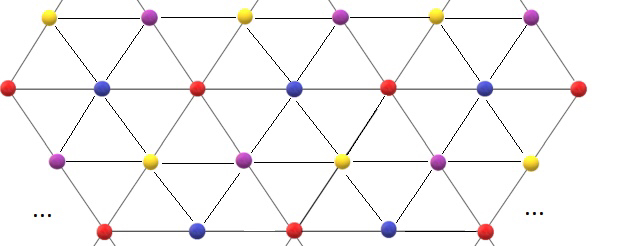
\includegraphics[width = 14cm]{Figure2.1.png}
\end{center}
Consider the following triangular lattice points where each adjacent points are 1 unit from each other. Suppose the 3 frogs are on 3 adjacent lattice points which form an equilateral triangle with sides length 1 initially. The frogs are on lattice points with three different colours. Note that after each jump, a frog will always land on a lattice point which has the same colour as its original point. But for an equilateral triangle with sides length of 10 units, the three vertices must be lattice points having the same colour. Therefore it is not possible.
\begin{flushright}
\textbf{7 marks}
\end{flushright}




\subsection*{\mybox{Problem 4 :}}
In chess, a knight moves either two squares vertically and one square horizontally, or two squares horizontally and one square vertically in each move. Suppose a knight can visit every squares on a $4 \times n$ chessboard exactly once without repeating. Find all the possible values of $n$.

\begin{flushright}
\textbf{Problem posed by}
\textcolor{RoyalBlue2}{\href{https://www.instagram.com/pepemaths/}{@pepemaths}}
\end{flushright}



\subsection*{\myboxs{Solution :}}
We claim that there are no possible values of n.
 
 \begin{center}
     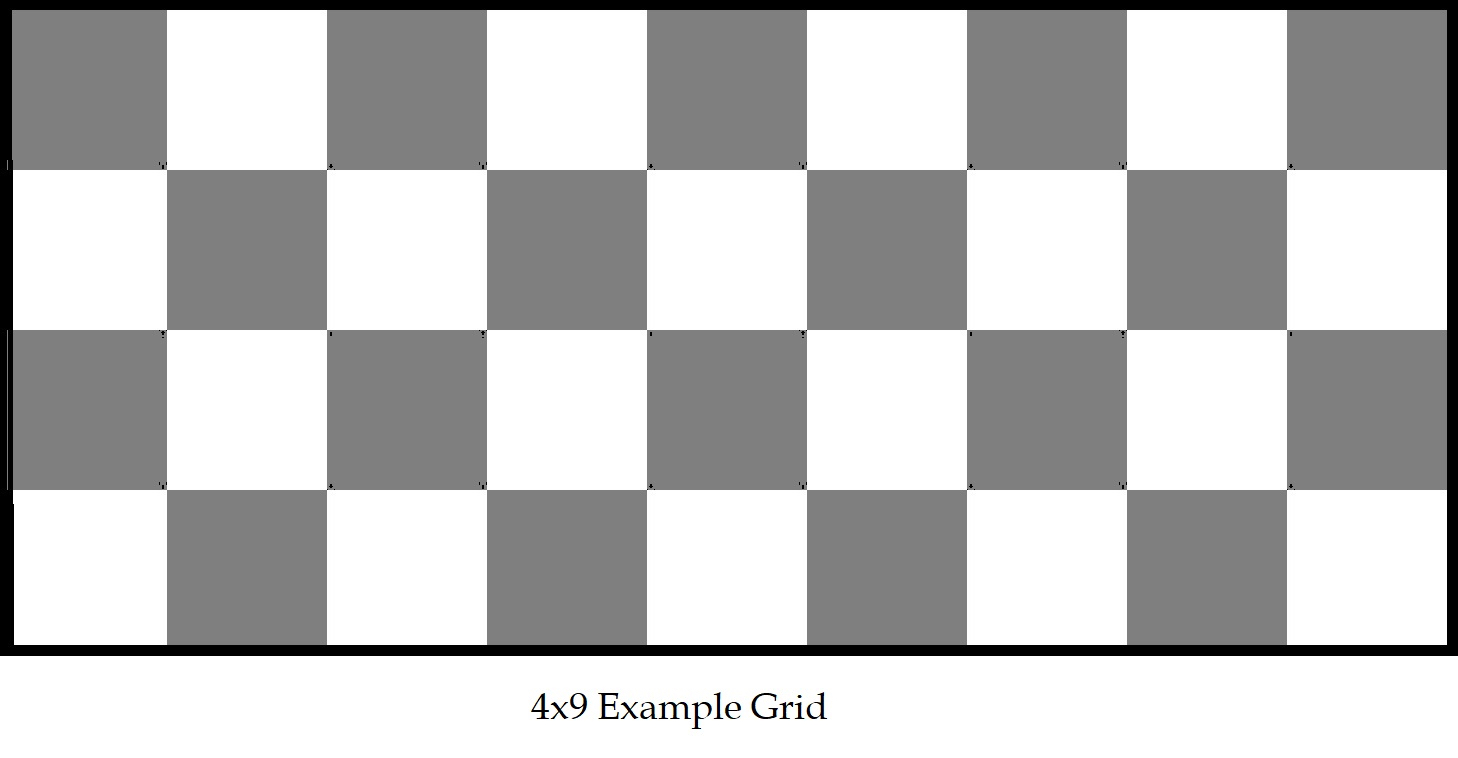
\includegraphics[width = 14cm]{Figure2.2.png}
 \end{center}
Colour the chessboard with black and white on alternate squares. Also, we call the squares on the first and forth row as peripheral squares (denoted by P), and those on the second and third row as centre squares (denoted as C). It is obvious that a knight must move from a black square to a white square, and a white square to a black square alternately  in each move. The knight always moves from a P square to a C square. It could move from a C square to either a C square or a P square, but since there are equal numbers of C squares and P squares,  if in one move, the knight moves from a C square to another C square, the there won't be enough C square for the knight to move to after every P squares. Therefore the knight must move from a P square to a C square, and a C square to a P square alternately  in each move. This is only possible if all the P squares are black and all the C squares are white, or all the P squares are white and all the C squares are black, which are both contradictory. So the knight can never visit every squares on a $4 \times n$ chessboard exactly once without repeating.


\subsection*{\mybox{Problem 5 :}}
People from 80 countries participated in the $1^{\textmd{st}}$ round of IGMO. In order to ensure that participants from any of the 80 countries can travel to any one of the remaining 79 countries by at most 2 flights, the countries have an agreement such that among the 80 countries, each country's airport connects to at least $n$ other countries' airport. 
\begin{itemize}
    \item Find the minimum value of $n$, proving that it is the minimum
    \item Prove that for this minimum $n$, if there isn't a direct flight between 2 countries, then there are at least 2 paths that require 2 flights between the countries
\end{itemize}
Note: For two airports $A$ and $B$ to be connected, it must be possible to have a flight from $A$ to $B$ and a flight from $B$ to $A$. This adds 1 to both the tallies of connections from the airports. Also note that for this problem, each country has only 1 airport.


\begin{flushright}
\textbf{Problem posed by}
\textcolor{RoyalBlue2}{\href{https://www.instagram.com/saitejasomu/}{@saitejasomu}} , \textcolor{RoyalBlue2}{\href{https://www.instagram.com/pepemaths/}{@pepemaths}} and \textcolor{RoyalBlue2}{\href{https://www.instagram.com/creative_math_/}{@creative\_math\_}}
\end{flushright}



\subsection*{ \myboxs{Solution :}}
Inspired by Ore's Theorem, we claim $n = 40$ is the minimum value of $n$. Let's then prove that $n = 39$ is impossible. Consider two groups of countries,
\begin{center}
    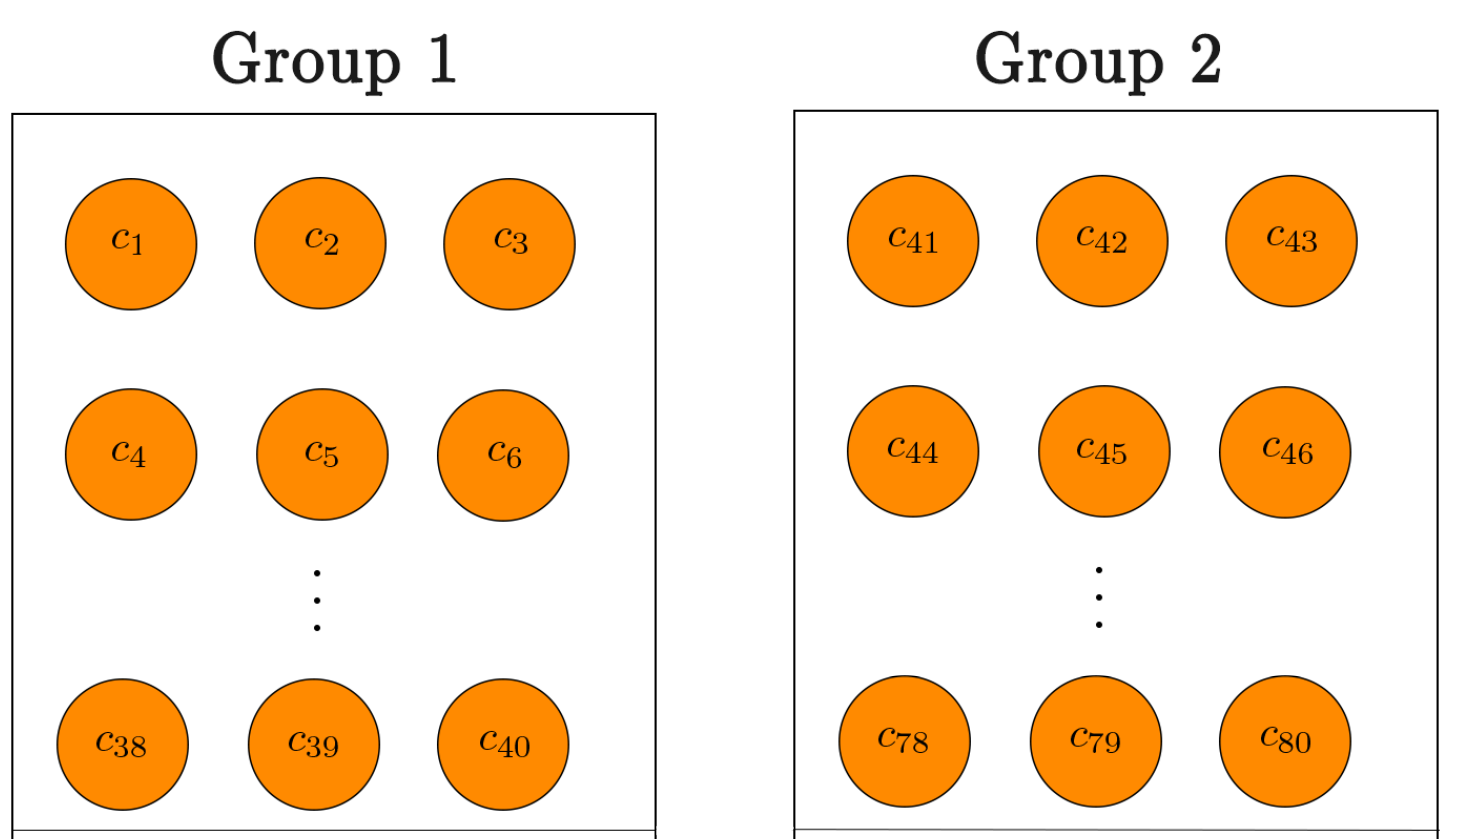
\includegraphics[width=16cm]{Figure 2.5.png}
\end{center}
The groups are arranged such that for any country $c_i$ in Group 1, each country it has a flight to is also in Group 1. This means that there exists a flight from $c_i$ to $c_1,c_2,c_3,\dots, c_{i-1}, c_{i+1}, \dots, c_{39}, c_{40}$. As it can have only 39 flights emerging from it, a country $c_j$ in Group 1 can only travel to a country $c_k$ in Group 1 and hence stays in Group 1. Hence $n= 39 $ cannot be our solution. \\ \\ Let us now examine $n = 40$. Suppose that we want to travel from country $c_A$ to $c_B$ in at most 2 flights, if there exists a connection from $c_A$ to $c_B$, we are done. If there doesn't, then we have 40 flights from $c_A$ and 40 flights from $c_B$, with no flight from $c_A$ to $c_B$ and vice versa. In total, there are 80 possible flights with 78 other countries to connect to, which means there exists a $c_n$ that has a flight from $c_A$ to it and a flight from $c_B$ to it(Pigeon-Hole Principle). As there exists a flight from $c_B$ to it, thee also exists a flight from $c_n$ to $c_B$ and we can move travel between $c_A$ and $c_B$ as so : $c_a \rightarrow c_n \rightarrow c_B$. Hence we can move from any country to the other in at most 2 flights and therefore $n = 40$. 
\begin{flushright}
\textbf{5 marks}
\end{flushright}
As $c_A$ and $c_B$ are not connected, there are 80 flights and 78 other countries. A country cannot have more than 1 flight between each other (there cannot be 2 flights from $c_A$ to $c_n$), there must exist 2 countries connected to both $c_A$ and $c_B$ (Pigeon-Hole Principle). Hence there are two paths from $c_A$ to $c_B$ and both require 2 flights.
\begin{flushright}
\textbf{2 marks}
\end{flushright}




\newpage
\section*{Geometry}




\subsection*{\mybox{Problem 1 :}}
A non-rectangular trapezoid is called a "Pepe trapezoid" if
\begin{enumerate}
\item It has integral side lengths AND
\item An ellipse with integral lengths of semi-major axis and semi-minor axis can be inscribed in the trapezoid such that the major axis or minor axis of the ellipse is perpendicular to the bases of the trapezoid.
\end{enumerate}
Prove or disprove that there exists infinitely many non-similar Pepe trapezoids.

\begin{flushright}
\textbf{Problem posed by}
\textcolor{RoyalBlue2}{\href{https://www.instagram.com/pepemaths/}{@pepemaths}}
\end{flushright}




\subsection*{\myboxs{Solution : }}
Suppose an ellipse is inscribed in an isosceles trapezoid $WXYZ$ with bases $WX$ and $YZ$ ($YZ>WX$). The lateral sides $XY$ and $ZW$ are equal. We denote the length of axis perpendicular to the bases as $2a$, the length of axis parallel to the bases as $2b$, respectively. Let $WX=s$, $YZ=t$, $XY=ZW=u$.

Height of the trapezoid is $\sqrt{u^2-(\frac{t-s}{2})^2}=\frac{\sqrt{4u^2-(t-s)^2}}{2}$. So
\begin{equation}\label{eq1}
a=\frac{\sqrt{4u^2-(t-s)^2}}{4}
\end{equation}

Then apply an affine transformation which dilates/contracts the figure along the major axis of the ellipse with a scale of $\frac{b}{a}$. The ellipse is transformed to a circle with radius $b$. Suppose points $W$, $X$, $Y$, $Z$ are transformed to $W'$, $X'$, $Y'$, $Z'$, respectively. Note that after the transformation, $W'X'=s$, $Y'Z'=t$, $X'Y'=Z'W'$. Moreover, $W'X'Y'Z'$ is a tangential trapezoid, by Pitot's theorem, $W'X'+Y'Z'=X'Y'+Z'W'$. Hence, $X'Y'=Z'W'=\frac{s+t}{2}$. Height of this triangle is $\sqrt{(\frac{s+t}{2})^2-(\frac{t-s}{2})^2}=\sqrt{st}$. So
\begin{equation}\label{eq2}
b=\frac{\sqrt{st}}{2}
\end{equation}

So a Pepe trapezoid is a trapezoid which $u$, $s$, $t$, $\frac{\sqrt{4u^2-(t-s)^2}}{2}$ and $\frac{\sqrt{st}}{2}$ are all integers. If is easy to verify that if $u=m^2+n^2$, $s=2n^2$, $t=2m^2$, where $m$ and $n$ are positive integers such that $m>n$, then $\frac{\sqrt{4u^2-(t-s)^2}}{4}=mn$,  $\frac{\sqrt{st}}{2}=mn$, which are also integers. By substituting different $m$ and $n$, we can generate infinitely many non-similar Pepe trapezoids.







\subsection*{\mybox{Problem 2 :}}
If $ABCD$ is a cyclic quadrilateral; $N_1$, $N_2$, $N_3$ and $N_4$ are the nine-point centres of $\triangle ABC$, $\triangle BCD$, $\triangle CDA$ and $\triangle DAB$, respectively. A circle with $AD$ as diameter meets $CD$ again at point $E$. Another circle with $AB$ as diameter meets $BC$ again at point $F$. Prove that $N_1$, $N_2$, $N_3$ and $N_4$ are concyclic and their circumcircle is bisected by line $EF$.

\begin{flushright}
\textbf{Problem posed by}
\textcolor{RoyalBlue2}{\href{https://www.instagram.com/pepemaths/}{@pepemaths}}
\end{flushright}



\subsection*{\myboxs{Solution :}}
\begin{center}
    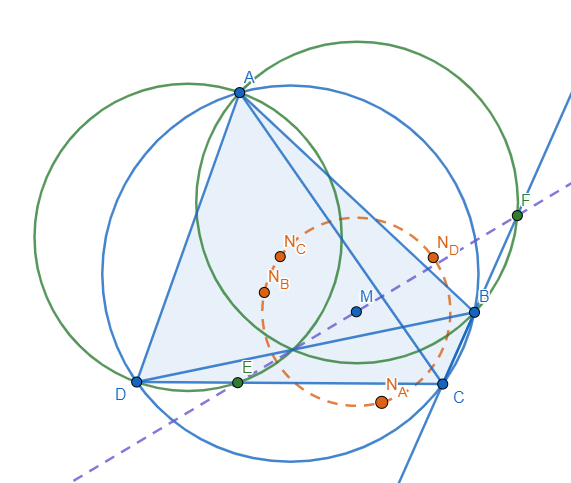
\includegraphics[width = 12cm]{Figure1.2.png}
\end{center}
We shall prove this using complex numbers. Introduce a complex plane. Let 0 be the centre of the circumcircle of ABCD, and let the circle be a unit circle. $n_1=\frac{a+b+c}{2}$, $n_2=\frac{b+c+d}{2}$, $n_3=\frac{c+d+a}{2}$, $n_4=\frac{d+a+b}{2}$. Let $m=\frac{a+b+c+d}{2}$, it is easy to verify that $|n_1-m|=|n_2-m|=|n_3-m|=|n_4-m|=\frac{1}{2}$. So $N_1$, $N_2$, $N_3$ and $N_4$ are concyclic. The centre of the circumcircle is point $M$, represented by $m=\frac{a+b+c+d}{2}$, and the radius of the circle is $\frac{1}{2}$. 

Note that $AE$ is perpendicular to $CD$, $AF$ is perpendicular to $BC$, so line $EF$ is the Simson line of $\triangle BCD$ with pole $A$. By a well known property of Simson line, we know that $EF$ passes through the mid-point of $A$ and the orthocentre of $\triangle BCD$, which is represented by $\frac{a+(b+c+d)}{2}=\frac{a+b+c+d}{2}$. So $EF$ passes through the centre of the circumcircle of $N_1 N_2 N_3 N_4$. It bisects the circumcircle.  


\subsection*{\mybox{Problem 3 :}}
For any given ellipse $\omega$, let $P$ be a point external to it. $A$ and $B$ are points on $\omega$ such that $PA$ and $PB$ are tangent to $\omega$. $C$, $D$ and $E$ are points on $\omega$ such that $AC=CD=DE=EB$. Lines $PC$, $PD$, $PE$ meets $\omega$ again at points $F$, $G$, $H$, respectively. $M_1$, $M_2$, $M_3$ are mid-points of $CF$, $DG$ and $EH$, respectively. Prove that $P$, $A$, $B$, $M_1$, $M_2$ and $M_3$ lie on an ellipse.

\begin{flushright}
\textbf{Problem posed by}
\textcolor{RoyalBlue2}{\href{https://www.instagram.com/pepemaths/}{@pepemaths}}
\end{flushright}


\subsection*{\myboxs{Solution :}}
\begin{center}
    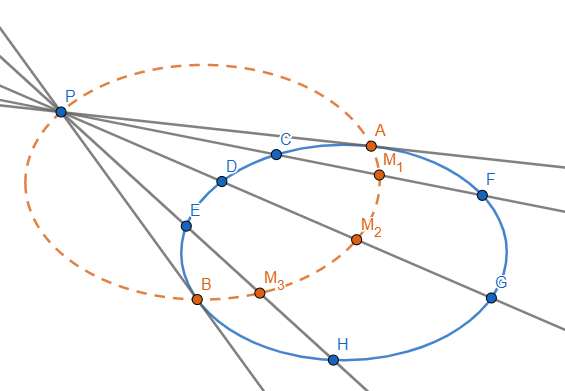
\includegraphics[width = 12cm]{Figure1.3.png}
\end{center}
Apply an affine transformation which transforms the ellipse into a circle. Suppose $P$, $A$, $B$, $C$, $D$, $E$, $F$, $G$, $H$, $M_1$, $M_2$, $M_3$ are transformed to $P'$, $A'$, $B'$, $C'$, $D'$, $E'$, $F'$, $G'$, $H'$, $M_1 '$, $M_2 '$, $M_3 '$, respectively. Note that $P'A'$ and $P'B'$ are tangent to the circle. $C'$, $D'$ and $E'$ are points on the circle such that $A'C'=C'D'=D'E'=E'B'$. Lines $P'C'$, $P'D'$, $P'E'$ meets the circle again at points $F'$, $G'$, $H'$, respectively. $M_1 '$, $M_2 '$, $M_3 '$ are mid-points of $C'F'$, $D'G'$ and $E'H'$, respectively.

Let $O$ be the centre of the circle. We claim that $O$, $P'$, $A'$, $B'$, $M_1 '$, $M_2 '$ and $M_3 '$ are concyclic. $\angle PAO=\angle PBO = 90^o$. $\angle PAO+\angle PBO = 180^o$. $O$, $P'$, $A'$, $B'$ are concyclic. $M_1 '$, $M_2 '$ and $M_3 '$ are mid-points of chords of the circle. $\angle P'M_1 'O=\angle P'M_2 'O=\angle P'M_3 'O$. So  $P'$, $O$, $M_1 '$, $M_2 '$, $M_3 '$ are concyclic. Overall,  $O$, $P'$, $A'$, $B'$, $M_1 '$, $M_2 '$ and $M_3 '$ are concyclic. Before the affine transformation,  $P$, $A$, $B$, $M_1$, $M_2$ and $M_3$ must lie on an ellipse.


\subsection*{\mybox{Problem 4 : }}
Some points are drawn on a plane such that the points do not have equal distances to each other. For each point, a line is drawn to connect it with its nearest point. Find the maximum possible number of  lines that a point is connected with.

\begin{flushright}
\textbf{Problem posed by}
\textcolor{RoyalBlue2}{\href{https://www.instagram.com/pepemaths/}{@pepemaths}}
\end{flushright}


\subsection*{\myboxs{Solution :}}
\begin{center}
    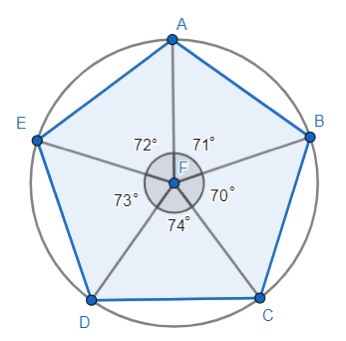
\includegraphics[width = 12cm]{Figure1.4.png}
\end{center}
We claim that the maximum possible number is $5$.

Refer to the figure consisting the vertices of a cyclic pentagon ($A$, $B$, $C$, $D$ and $E$). Let $F$ be a point slightly deviated from the circumcentre of the pentagon such that $AF$,$BF$, $CF$, $DF$ and $EF$ are not equal to each other, it is easy to verify that $A$, $B$, $C$, $D$ and $E$ should be connected with $F$. So there are five lines connected with $F$, hence it is possible to have $5$ lines connected to a point.

We shall show that $6$ is not possible. Consider any $3$ points, $A$, $B$ and $C$.  Suppose there are 2 lines connected to $B$. WLOG, assume $AB<BC$.  $B$ must be the nearest point of $A$, so there is a line connecting $A$ and $B$, and $AB<AC$. If not, then $AC<AB<BC$, the nearest point of $C$ must be $A$, then only one line is connected to $B$, which contradicts with our assumption.

By assumption, there is also a line connecting $B$ and $C$, since $AB<BC$, the nearest point of $B$ cannot be $C$, so the nearest point of $C$ must be $B$, therefore $BC<AC$. Overall we have, $AB<BC<AC$. So $\angle ABC>60$. If there are 6 lines connecting to a point, all the angles formed by adjacent lines are $>60^{\circ}$, the sum of the 6 angles are greater than $360^{\circ}$, which is impossible.


\subsection*{\mybox{Problem 5 : }}
Let $I$, $H$, $O$ be the incentre, orthocentre and circumcentre of $\triangle ABC$ respectively. $D$ is the circumcentre of $\triangle AIC$. $H$ is reflected along $BC$ and $AB$ to $E$ and $F$ respectively. Prove that $D$, $O$, $F$ are collinear if and only if $DE$ is perpendicular to $EF$.

\begin{flushright}
\textbf{Problem posed by}
\textcolor{RoyalBlue2}{\href{https://www.instagram.com/pepemaths/}{@pepemaths}}
\end{flushright}

\subsection*{\myboxs{Solution :}}
\begin{center}
    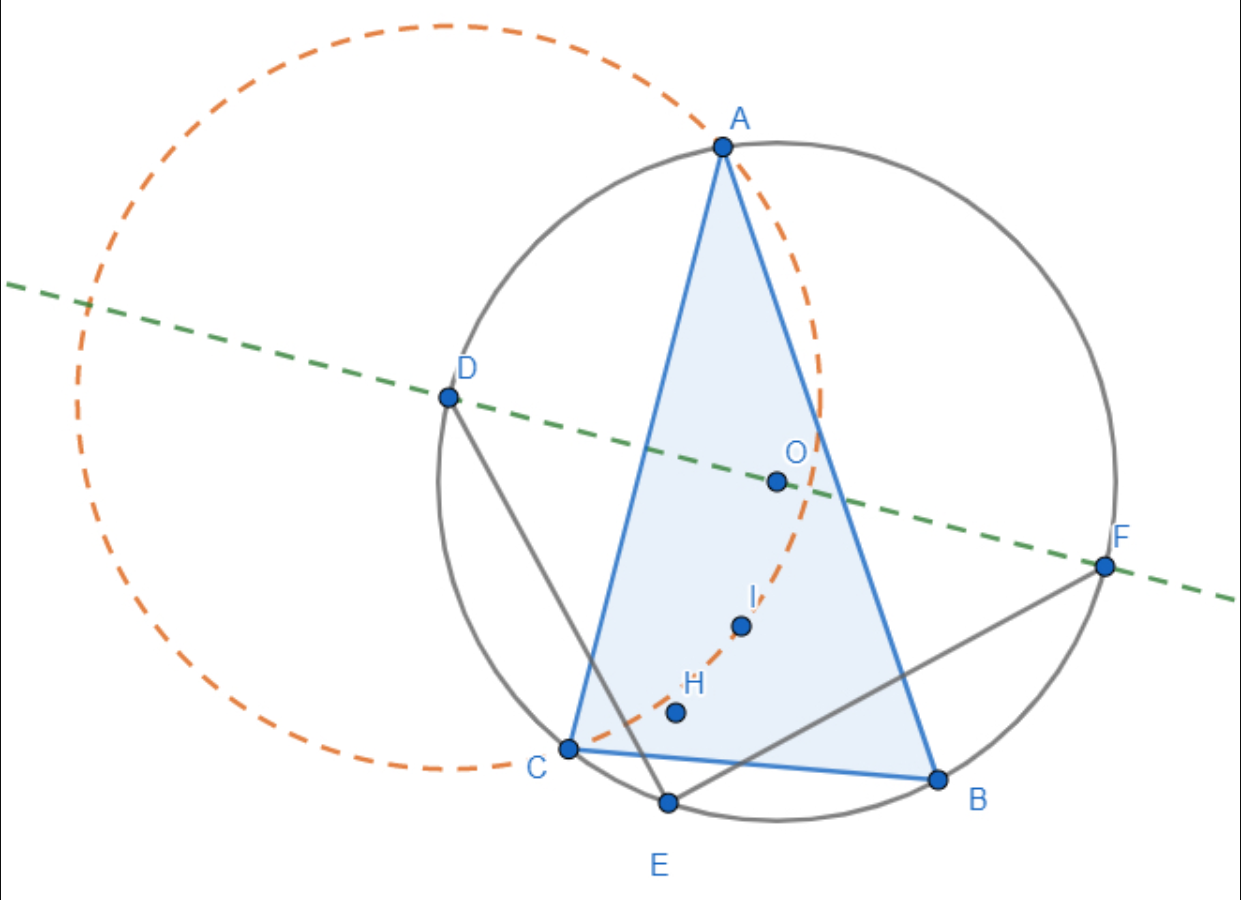
\includegraphics[width = 10cm]{Figure 5.png}
\end{center}
By incentre-excentre lemma, $D$ is on the circumcircle of $\triangle ABC$. Also, it is a well known property of orthocentre that $E$ and $F$ are on the circumcircle of $\triangle ABC$. So, $D$, $O$, $F$ are collinear if and only if $DF$ is the diameter of circumcircle of $\triangle ABC$ if and only if DE is perpendicular to EF.



\subsection*{\mybox{Problem 6 : }}
A sphere of radius $r$ can be inscribed in a tetrahedron. The distances between the centroid of the tetrahedron and its four faces are $w$, $x$, $y$ and $z$. Prove that $wxyz \ge r^4$.

\begin{flushright}
\textbf{Problem posed by}
\textcolor{RoyalBlue2}{\href{https://www.instagram.com/pepemaths/}{@pepemaths}}
\end{flushright}


\subsection*{\myboxs{Solution :}}
Let the tetrahedron be $ABCD$ and $G$ be the centroid. Let the areas of $\triangle BCD$, $\triangle CDA$, $\triangle DAB$ and $\triangle ABC$ be $s_1$, $s_2$, $s_3$ and $s_4$ respectively. Let the distances between $G$ and $\triangle BCD$, $\triangle CDA$, $\triangle DAB$ and $\triangle ABC$ be $w$, $x$, $y$ and $z$ respectively. Let $V$ be the volume of the tetrahedron.

Note that the volumes of tetrahedrons $GBCD$, $GCDA$, $GDAB$ and $GABC$ are equal. We have $\frac{w s_1}{3}=\frac{x s_2}{3}=\frac{y s_3}{3}=\frac{z s_4}{3}$.

Also, $V=\frac{w s_1}{3}+\frac{x s_2}{3}+\frac{y s_3}{3}+\frac{z s_4}{3}=\frac{r s_1}{3}+\frac{r s_2}{3}+\frac{r s_3}{3}+\frac{r s_4}{3}=\frac{r(s_1 + s_2 + s_3 + s_4)}{3}$.
$$\frac{w s_1}{3}=\frac{x s_2}{3}=\frac{y s_3}{3}=\frac{z s_4}{3}=\frac{1}{4}\frac{r(s_1 + s_2 + s_3 + s_4)}{3} \ge \frac{r\sqrt[4]{s_1  s_2  s_3  s_4}}{3} $$
$$w s_1 = x s_2 = y s_3 = z s_4 \ge r \sqrt[4]{s_1  s_2  s_3  s_4}$$
$$w s_1  x s_2  y s_3  z s_4 \ge (r \sqrt[4]{s_1  s_2  s_3  s_4})^4=r^4 s_1  s_2  s_3  s_4$$
$$wxyz \ge r^4$$


\newpage

\section*{Number Theory}
\subsection*{\mybox{Problem 1 :}}
For any natural number $n$ and all natural numbers $d$ dividing $2n^2$ show that $n^2+d$ is not the square of a natural number 

\begin{flushright}
\textbf{Problem posed by}
\textcolor{RoyalBlue2}{\href{https://www.instagram.com/mathinity/}{@mathinity}}
\end{flushright}



\subsection*{\myboxs{Solution :}}

Suppose that
$$\exists_{x \in \mathrm{N}}: n^{2}+d=x^{2}$$
since $d$ divides $2 n^{2},$ we know that
$$\exists_{k \in \mathbb{N}}: 2 n^{2}=d k$$
By multiplying both sides of the first equation by $k^{2}$ we obtain
$$k^{2} x^{2}=k^{2} n^{2}+k^{2} d=n^{2}\left(k^{2}+2 k\right)$$
Above equation implies that $k^2+2k$ is a square number. This is a contradiction as $$k^2 < k^2+2k < (k+1)^2$$ and a square cannot lie between 2 consecutive squares.

\subsection*{\myboxs{Alternative Solution :}}
if $d|2n^2$, then we have $dk = 2n^2$. Suppose now that 
$$ n^2+d = m^2 $$
For some $m \in \mathbb{N}$. Clearly, $m^2 > n^2$. Multiplying both sides of the equation by $k$, we get 
$$ n^2k+dk = m^2k $$
$$ n^2(k+2) = m^2k \Rightarrow \frac{n^2}{m^2} = \frac{k}{k+2} $$
If $k$ is even, $k = 2a$ for some $a \in \mathbb{N}$, then we'd have 
$$ \frac{n^2}{m^2} = \frac{a}{a+1} $$
As $a$ and $a+1$ are co-prime, $n^2 = a$ and $m^2 = a+1$, but this can't happen as squares must be at least 3 apart. \\ If $k$ is odd, then $k$ and $k+2$ are co-prime and hence $n^2 = k $ and $m^2 = k+2$ which is again a contradiction. To prove that two consecutive odd numbers are co-prime, assume that they share a common prime $p_1$ in their factorization. Then we'd have 
$$ k+2 = xp_1 \quad, \quad k = yp_1 $$
Subtracting, we have 
$$ p_1(x-y) = 2 $$
As $p_1 >  2 $ (as they're odd), this is a contradiction








\begin{flushleft}
\subsection*{\mybox{Problem 2 :}}
Let's define a function $\phi:\mathbb{N}\rightarrow \mathbb{N}$, where $0\notin\mathbb{N}$, as follows
\[\phi(n)=\sum_{k=1}^{n}k!\]
 
 Let $\mathbb{V}$ be defined as the set of all triplets $(x,y,z) \in \mathbb{N}$ such that $\phi(x) = y^{z+1}$. For a triplet $x,y,z$ (denoted by $v$) in $\mathbb{V}$, we define
 \[f_{v}(n)=8\left[\frac{xy}{8}\right]\lfloor \sqrt{n}\rfloor+\frac{zn}{z+x-y}.\]
 \begin{flushright}
 ($[x]$ is \textbf{fractional part}  of $x$ and $\lfloor x \rfloor$ is greatest integer less than $x$)
 \end{flushright}
 
 Show that for any $v\in\mathbb{V}\text{ and }m\in\mathbb{N}$ the sequence 
 \[m,\ f_{v}(m),\ f_{v}(f_{v}(m)),\ f_{v}(f_{v}(f_{v}(m))),...\]
 contains at least one square of a natural number. Please note that $[x]$ here refers to the \textbf{fractional part} of $x$, it can also be denoted as $\{x\}$ but it is denoted as $[x]$ here.
 
 
 
 \begin{flushright}
\textbf{Problem posed by}
\textcolor{RoyalBlue2}{\href{https://www.instagram.com/mathinity/}{@mathinity}}
\end{flushright}
 
 
 
 
 
 
\subsection*{\myboxs{Solution 2 :}}
Firstly let's find all elements of $\mathbb{V}$. Let's do 2 cases
\begin{enumerate}[label=\arabic*.]
    \item  $z=1$. We can notice that 
    \[\forall_{x\geq4}:\phi(x)\equiv 3\ \text{(mod }10)\]
    and 
    \[\forall_{y\in\mathbb{N}}:y^2\not\equiv3\ \text{(mod }10),\]
    Hence all $(x,y,1)$ for $x\geq 4$ can't be an element of $\mathbb{V}$. By checking $(1,y,1),(2,y,1)\text{ and }(3,y,1)$ we find out that the only triples that satisfy the equation $\phi(x)=y^{z+1}$ are 
    \[(1,1,1)\quad \text{ and }(3,3,1)\]
    \item $z>1$. Of course if we set $x=y=1$, then we have infinitely many new elements of $\mathbb{V}$
    \[\forall_{z>1}:(1,1,z)\in\mathbb{V}\]
    Let's set $x,y>1$ and split this one into 3 cases\begin{enumerate}[label=\textbullet]
        \item $x\in\{2,...,6\}$. We can notice, that $\phi(x)$ is divisible by 3, but not by 27, so for $x\in\{2,...,6\}$, $(x,y,z)\notin\mathbb{V}$. 
        \item $x=7$. We can see that $\phi(7)=5913$ is divisible by 73, but not by $73^2$, so $(7,y,z)$ can't be an element of $\mathbb{V}$.
        \item $x>7$. We can observe, that $\forall_{n>8}:n!\equiv0\text{ (mod }27)$, so 
        \[\forall_{x>7}:\phi(x)\equiv\phi(8)\equiv46233\equiv9\text{ (mod }27).\]
        Hence $\phi(x)$ is divisible by 9, but not by 27, so for $x>7$, $(x,y,z)\notin\mathbb{V}$.
    \end{enumerate}
\end{enumerate}
It follows that 
\[\mathbb{V}=\{(1,1,z)\in\mathbb{N}^3:z\in\mathbb{N}\}\cup\{(3,3,1)\}\]

Let's take $v\in\mathbb{V}$ and put it into the definition of $f_v(n)$. We can see that 
\[\forall_{v\in\mathbb{V}}:f_v(n)=8\left[\frac{xy}{8}\right]\lfloor\sqrt{n}\rfloor+\frac{zn}{z+x-y}=\lfloor\sqrt{n}\rfloor+n=:f(n)\]

Let's set $m\in\mathbb{N}$. We can define $k:=\lfloor\sqrt{m}\rfloor$. It means that $m=k^2+j$ for some $j\in\{0,1,...,2k\}$. Let's break this up into 2 cases\begin{enumerate}[label=\arabic*.]
\item $j\in\{0,1,...,k\}$. To prove the thesis we'll need the following lemma
\begin{lemma}
    If $f^{r}(m)=f(f^{r-1}(m))$, then the equation
    \[f^{2r}(m)=(k+r)^2+(j-r)\]
    holds true for all $r\in\{0,...,j\}$
\end{lemma}
\begin{proof}
    We will perform a proof by induction with respect to $r$. If we set $r=1$, then we obtain
    \[f^2(m)=f(f(m))=f(m+k)=f(k^2+k+j)=k^2+k+j+\lfloor\sqrt{k^2+k+j}\rfloor.\]
    Since $j\in\{0,1,...,k\}$, we have $k^2+k+j< k^2+2k+1=(k+1)^2$, so
    \[f^2(m)=k^2+k+j+\lfloor\sqrt{k^2+k+j}\rfloor=k^2+2k+j=(k+1)^2+(j-1)\]
    Now that we have our base case, we can do the induction step. Let's assume that the lemma is true for $r$. We need to prove the lemma for $r+1$. We have
    \begin{align*}
        f^{2(r+1)}(m)&=f(f(f^{2r}(m)))=f(f((k+r)^2+j-r))\\
        &=f((k+r)^2+j-r+\lfloor\sqrt{(k+r)^2+j-r}\rfloor)=:F
    \end{align*}
    Like in the base case we can see that $(k+r)^2+j-r<(k+r+1)^2$, so
    \begin{align*}
    F&=f((k+r)^2+j-r+k+r)=f((k+r)^2+k+j)\\
    &=(k+r)^2+k+j+\lfloor\sqrt{(k+r)^2+k+j)}\rfloor
    \end{align*}
    Once again we can notice that $(k+r)^2+k+j<(k+r+1)^2$, so
    \begin{align*}
    F&=(k+r)^2+k+j+k+r=(k+(r+1))^2+(j-(r+1))
    \end{align*}
\end{proof}
    By the \textbf{Lemma 1.1} we know that $f^{2j}(m)$ is a square of a natural number.
    \item $j\in\{k+1,k+2,...,2k\}$. By considering $f(m)$ instead of $m$ we reduce this case to the $1^{\textmd{st}}$ case. Hence proved.
    
\end{enumerate}
\end{flushleft}



\subsection*{\mybox{Problem 3 : }}
Find $\ a,b,c,d \in \mathbb{N} $ such that: $\ a+2^{b}+3^{c}=3d!+1$
and exist $\ p,q $ prime such that :
$\ a=(p+1)(2p+1)=(q+1)(q-1)^2 $

\begin{flushright}
\textbf{Problem posed by}
\textcolor{RoyalBlue2}{\href{https://www.instagram.com/creative.math_solving/}{@creative.math\_solving}}
\end{flushright}
\subsection*{\myboxs{Solution :}}
We have 
\begin{align*}
(p+1)(2p+1)&=(q+1)(q-1)^2 \\
2p^2+3p&=q^3-q^2-q \\
p(2p+3)&=q(q^2-q-1)
\end{align*}
Thus $p\mid q^2-q-1$ and $q\mid 2p+3$ indeed $2p+3=qk\iff p=\frac{qk-3}{2}$. Notice $q\equiv \frac{3}{k} \mod \frac{qk-3}{2}$
\begin{align*}
q^2-q-1&\equiv 0\mod \frac{qk-3}{2} \\
\frac{9}{k^2}-\frac{3}{k} &\equiv 1\mod \frac{qk-3}{2} \\
9-3k &\equiv k^2\mod \frac{qk-3}{2} \\
\end{align*}
Thus $k^2+3k-9\ge \frac{qk-3}{2}$ indeed $2k+6-\frac{15}{k}\ge q$ indeed $2k+6\ge q$ thus $k\ge \frac{q-6}{2}$

Now 
\begin{align*}
2p^2+3p&=q^3-q^2-q \\
\frac{(qk-3)^2}{2}+\frac{3}{2} (qk-3) &= q^3-q^2-q \\
(q\left(\frac{q-6}{2}\right)-3)^2+3(q\left(\frac{q-6}{2}\right)-3) &\le 2q^3-2q^2-2q \\
\frac{q^4}{4}-3q^3+\frac{15q^2}{2}+9q &\le 2q^3-2q^2-2q \\
\frac{q^4}{4}-5q^3+\frac{19q^2}{2}+11q &\le 0 \\
\end{align*}
In fact the trivial without using computing bound is $25>q$. But let us use computing and so $17\ge q\ge 5$.

Nice, now we have $q\in\{5,7,11,13,17\}$ checking when $2p^2+3p=q^3-q^2-q$ we get $(p,q)=(31,13)$ i.e $a=2016$.


Thus we have
$$2015+2^b+3^c=3d!$$
With $2015<3d!$ we get $d\ge 7$. Also $2+(-1)^b\equiv 0\mod 3$ yielding $b$ is even. So $b\ge 2$ and thus $-1+(-1)^c\equiv 0\mod 4$ yielding $c$ is even i.e $(b,c)=(2x,2y)$. Now write as $2015+4^x+9^y=3d!$ so
$$4^x\equiv 1\mod 9$$
Thus $x=3u$. Yielding $2015+64^u+9^y=3d!$. So
$$2^{y}\equiv 0 \mod 7$$
Which is impossible, so there are no solutions.










\subsection*{\mybox{Problem 4 :}}
Let $k$ be a positive real number such that $\lfloor kn^2 \rfloor$ is perfect square for all $n\in \mathbb{N}$ Show that $k$ must be a perfect square.
\begin{flushright}
\textbf{Problem posed by} \textcolor{RoyalBlue2}{\href{https://www.instagram.com/creative.math_solving/}{@creative.math\_solving}}
\end{flushright}








\subsection*{\myboxs{Solution :}}
If $k$ is irrational, let $p>1$ be any positive integer. If $k$ is rational, let $p$ be a prime not dividing its denominator.
Let $m$ be the smallest positive integer such that $\lfloor kp^{2m}\rfloor>p$. Let $\lfloor kp^{2m+2n}\rfloor=a_n^2$ for all integers $n\ge0$.
$$a_{n+1}^2=\lfloor kp^{2m+2n+2}\rfloor\ge p^2\lfloor kp^{2m+2n}\rfloor=p^2a_n^2$$
As $a_n>p$ for all $n$
\begin{align*}
a_{n+1}^2&=\lfloor kp^{2m+2n+2}\rfloor\\
&\le kp^{2m+2n+2}\\
&<p^2(kp^{2m+2n}-1)+2p^2+1\\
&<p^2a_n^2+2pa_n+1\\
\end{align*}
From the two inequalities above $p^2a_n^2\le a_{n+1}^2<p^2a_n^2+2pa_n+1\implies pa_n\le a_{n+1}<pa_n+1\implies pa_n=a_{n+1}$ which by induction means $a_n=p^nq$ for all $n$, where $q$ is some positive integer.
\begin{align*}\lfloor kp^{2m+2n}\rfloor&=p^{2n}q^2\\
p^{2n}q^2-1<kp^{2m+2n}&\le p^{2n}q^2-1\\
q^2-\frac1{p^{2n}}<kp^{2m}&\le q^2\end{align*}
By taking $n$ to infinity, $kp^{2m}=q^2$ so $kp^{2m}$ must be a perfect square, so $k$ must be too.
\end{document}





